\chapter{Concepts clé}
Symfony2 est un framework MVC PHP open source développé par l'entreprise SensioLabs et est l'un des framework les plus utilisé dans le monde du web. Il dispose d'une très grande communauté et d'un large panel de modules (\og{}Bundles\fg{}) développés par cette communauté.
\paragraph{}
Dans ce chapitre, je ne vais pas revenir sur les concepts de base et tous les compsants de Symfony 2 (controlleur, routing, etc) mais je vais vous présenter quelque concepts clé utilisé par Symfony 2 qui permettent justement le fait couplage d'Open Orchestra.
\section{Bundles}
Un bundle Symfony est un repertoire qui contient un ensemble de fichiers structurés (contrôleur, entité commande, listener, formulaire) qui permettent d'implémenter une fonctionnalité réutilisable dans n'importe quelle application Symfony2. Sous Symfony2 presque tout est découpé en bundle même le kernel du framework.
\paragraph{}
Les différentes classes et fichiers d'un bundle sont organisé selon l'architecture suivante : 

\begin{verbatim}
      Bundle/
           Command/  
           Controller/
           DependencyInjection/
           EventListener/
          Tests/
          Ressources/
                    config/
                    public/
                    translations/
                    views/
\end{verbatim}
\begin{itemize}
\item[]
\item \textbf{Command} Contient les commandes du bundles
\item \textbf{Controller} Contient les contrôleurs du bundles
\item \textbf{DependencyInjection} Contient les classes qui peuvent importer la configuration de servcies, ajouter des passes de compilation, je reviendrais plus en détail sur ce repertoire par la suite
\item \textbf{EventListener} Les listeners d'évènements du bundle
\item \textbf{Tests} Tests unitaires et fonctionnels du bundle
\item \textbf{Resources/config/} Configuration du bundle (routage, déclarations de service, etc)
\item \textbf{Resources/views/} Templates (vues) utilisé dans le bundle
\item \textbf{Resources/public/} Ressources web (js, css, images, etc)
\end{itemize}
\paragraph{}
Pour permettre une plus grande flexibilité un bundle peut définir sa propre configuration (fichiers du répertoire config) qui peut être surcharger par la configuration générale de l'application qui utilise le bundle.
http://symfony.com/fr/doc/current/components/dependency_injection/workflow.html
TODO Les passes de compilation
\section{Conteneur de service}

\subsection{Service}
\paragraph{}
Un service est simplement un objet qui réalise une fonction spécifique comme par exemple envoyer un mail. L'avantage d'avoir de nombreux services pour gérer les différentes fonctionnalités de son application est de permettre la séparation de son code et donc une plus grande flexibilité.
\paragraph{}
Avec Symfony2, pour créér un service il suffit de le déclarer dans un fichier de configuration (yaml, xml, php), en générale ce fichier est appellé \verb?services.yml?
et de charger ce fichier lors du chargement du bundle (Extension @TODO parlé du chargement du bundle).
Lorsque l'on déclare un service, il faut indiquer sa classe et eventuellement les differents arguments dont a bessoin le service.
\paragraph{}
Par exemple, le fichier de configuration yaml suivant déclare deux services, \verb?service2? et \verb?service2?.
La classe \verb?Service1? a bessoin d'une instance de \verb?Service2? pour cela, on peut utiliser la syntaxe \verb?@service2? qui indique au conteneur de service de chercher un service appellé \verb?service2 et de transmettre une instance au constructeur de \verb?Service2?

\begin{verbatim}

  services:
      service2:
          class: "\MonBundle\Service2"
      service1:
          class: "\MonBundle\Service1"
          arguments: ["@service2"]
          tags:
                - { name: tag }

\end{verbatim}
\paragraph{}
Pour finir, lorsque l'on déclare un service, il peut être taggé comme le montre l'exemple ci-dessus avec le paramètre \verb?tags?.
L'intérét d'avoir des services taggé et de pouvoir récupérer tous les services qui posséde un certains tag. c'est notamment utilisé par le pattern stratégie, que je vous ai présenté dans la section précédente, pour récupérer les differentes stratégie.
\paragraph{}
Ce type d'architecture est appelé \og architecture orienté service \fg{} et n'est pas spécifique à Symfony ou même à PHP.
\subsection{Conteneur}
Les différents services sont géré par le conteneur de service. Le conteneur de service est un objet qui gère tous les services, récupération d'un service, instanciation d'un service, etc.
\paragraph{}
Par exemple, supposons que nous avons deux services (service1, service2) et que le service 1 a besoin du service2. Lorsque l'on fait appelle au service1 le schéma~\ref{conteneur} décrit le fonctionnement du conteneur de service pour récupérer le service.
		\begin{figure}[H]
        \begin{center}
          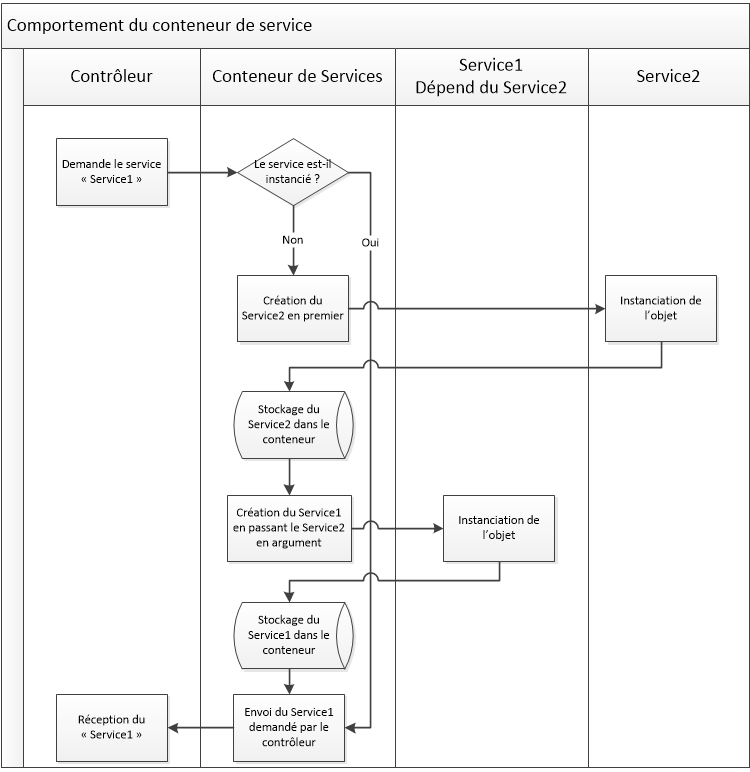
\includegraphics[scale=0.8]{images/conteneur_service}
        \end{center}
        \caption{Fonctionnement du conteneur de serveur lors de la demande d'un service}
        \label{conteneur}
      \end{figure}

\paragraph{}
Les différents services sont partagés au sein d'un conteneur, c'est-à-dire qu'un service est instancié une seul et unique fois à la première demande de celui-ci. Ce qui permet a  différents objet de manipuler la même instance d'un service tout au long de la requête.
